\subsection{Code Generator}

In this section you will learn how to implement the code generator for 
the target application. For simplicity, the code generator templates are placed
in the \texttt{org.eclipse.xtext.example.ql} project in a sub-package \texttt{generator}. 
Usually it would be better to create a separate project which contains the generator,
since the language is independent from a single target platform. It would
be possible to create different code generators for different target platforms,
and it would be better to implement each of them as separate projects.

Generator templates in Xtend are implementations of the \texttt{IGenerator}
interface:

\begin{lstlisting}[language=Java]
package org.eclipse.xtext.generator;

public interface IGenerator {
	/**
	 * @param input - the input for which to generate resources
	 * @param fsa - file system access to be used to generate files
	 */
	public void doGenerate(Resource input, IFileSystemAccess fsa);
}
\end{lstlisting}

\subsubsection {Dispatcher template}
\label{sec:dispatcherTemplate}

The code generator is invoked with a \texttt{Resource} instance, which holds a \texttt{Questionnaire}
instance. We have to generate multiple artifacts for each resource, so it is a common 
pattern to create a template class which serves as entry point and dispatches to other
template classes to create the artifacts. Usually one template per artifact is
created.

Create the class \texttt{Root.java} in 
package \texttt{org.eclipse.xtext.example.ql.generator}:

\begin{lstlisting}[language=Java]
package org.eclipse.xtext.example.ql.generator;

import javax.inject.Inject;

import org.eclipse.emf.ecore.resource.Resource;
import org.eclipse.xtext.generator.IFileSystemAccess;
import org.eclipse.xtext.generator.IGenerator;
import org.eclipse.xtext.xbase.compiler.JvmModelGenerator;

@SuppressWarnings("restriction")
public class Root implements IGenerator {
  @Inject
  JvmModelGenerator jvmModelGenerator;

  public void doGenerate(Resource input, IFileSystemAccess fsa) {
    // dispatch to other generators
    jvmModelGenerator.doGenerate(input, fsa);
  }
}
\end{lstlisting}

As a first generator to which is dispatched, we inject an instance of
\texttt{JvmModelGenerator}. This is a standard generator shipped with Xtext which
translates types inferred by the Jvm Model Inferrer to Java classes.
In our case, the Java class for Forms are generated by the
\texttt{JvmModelGenerator}. In JSF terms, we speek of the \emph{Backing Bean}.
 
Next, Xtext has to know that \texttt{Root} is the template that has to be invoked
as generator implementation. This has to be configured - you guessed right! - 
with Guice again. We need to add a configuration that binds the \texttt{IGenerator}
interface to the \texttt{Root} class.

Open class \texttt{QlDslRuntimeModule} and add this method:

\begin{lstlisting}[language=Java]
  @Override
  public Class<? extends IGenerator> bindIGenerator() {
    return Root.class;
  }
\end{lstlisting}

Now we are ready to add additional templates and register them in the
\texttt{Root} class.

\subsubsection{Output Configuration Provider}
\label{sec:outputConfigurationProvider}

In JSF applications all the web related content is normally placed under
\texttt{./WebContent} instead of \texttt{./src-gen}, which is mostly used as
output for java artifacts. We will adapt to this convention and seperate
generated java classes and jsf artifacts from each other. For that purpose add a class called
\texttt{JsfOutputConfigurationProvider} derived from
\texttt{OutputConfigurationProvider}
\footnote{\url{http://xtextcasts.org/episodes/15-output-configurations}} which
adds an additional \texttt{OutputConfiguration} pointing to the ouput directoy
\texttt{./WebContent} as shown in the listing below.

\begin{lstlisting}[language=Java]
package org.eclipse.xtext.example.ql.generator;

import java.util.Set;

import org.eclipse.xtext.generator.OutputConfiguration;
import org.eclipse.xtext.generator.OutputConfigurationProvider;

public class JSFOutputConfigurationProvider extends OutputConfigurationProvider {

  public final String WEB_CONTENT = "WebContent";

  /**
   * @return a set of {@link OutputConfiguration} available for the generator
   */
  public Set<OutputConfiguration> getOutputConfigurations() {
    Set<OutputConfiguration> outputConfigurations = super
        .getOutputConfigurations();

    OutputConfiguration webContent = new OutputConfiguration(WEB_CONTENT);
    webContent
        .setDescription("Read-only Output Folder for web generated application artifacts");
    webContent.setOutputDirectory("./WebContent");
    webContent.setOverrideExistingResources(true);
    webContent.setCreateOutputDirectory(true);
    webContent.setCleanUpDerivedResources(true);
    webContent.setSetDerivedProperty(true);
    outputConfigurations.add(webContent);

    return outputConfigurations;
  }
}
\end{lstlisting}

The interface \texttt{OutputConfiguration} provides several options to configure
the behavior of the so called \texttt{Outlet}. We use the defaults as in
\texttt{OutputConfigurationProvider} except its name, description and outputDirectoy.

Our \texttt{JsfOutputConfigurationProvider} has to be bound to the
\texttt{QlDslRuntimeModule} by overriding the method \texttt{configure}. 

\begin{lstlisting}[language=Java]
@Override public void configure(Binder binder) {
    super.configure(binder);
    binder.bind(IOutputConfigurationProvider.class)
        .to(JSFOutputConfigurationProvider.class).in(Singleton.class);
  }
 \end{lstlisting}
 
After this step we can refer to the additional \texttt{OutputConfiguration} in
generators by use of the constant \texttt{WEB\_CONTENT} defined in class
\texttt{JsfOutputConfigurationProvider}.

\subsubsection {JSF Generator}
\label{sec:jsfGenerator}

After creation of the class \texttt{Root} in section
\ref{sec:dispatcherTemplate} where we easily can
add new Generators and the defintion of the
\texttt{JsfOutputConfigurationProvider} in section \ref{sec:outputConfigurationProvider}
which prvides an output folder for JSF
artifacts, we use the \emph{New Xtend Class Wizard} to create a new Xtend class
called \texttt{JSFGenerator.xtend} in package \texttt{org.eclipse.xtext.example.ql.generator}.

This class will be our entry point to generate JSF related artifacts. The
\emph{New Xtend Class Wizard} provides the possibility to bind interfaces to the
new class by use of the \texttt{Add} button near the interface section.

\begin{center}
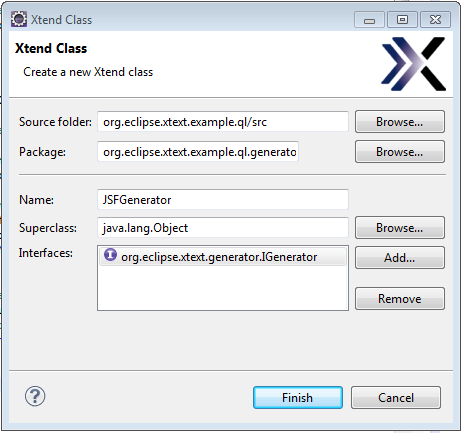
\includegraphics[width=8cm]{./images/chapter02/newXtendClassWizard.png}
\end{center}

As we want to create a new generator we add the interface
\texttt{org.eclipse.xtext.generator.IGenerator} to our new Xtend class.
After typing in the package, the name and the interface of our new Xtend class
as shown in the figure above, we can finish the
wizard so that the class shown in the following listing
will be created in our project.

\begin{lstlisting}[language=Java] 
package org.eclipse.xtext.example.ql.generator

import org.eclipse.xtext.generator.IGenerator
import org.eclipse.emf.ecore.resource.Resource
import org.eclipse.xtext.generator.IFileSystemAccess

class JSFGenerator implements IGenerator {
	
	override doGenerate(Resource input, IFileSystemAccess fsa) {
		throw new UnsupportedOperationException("TODO: auto-generated method stub")
	}
}
\end{lstlisting}

To get the created \texttt{JSFGenarator} executed we have to inject and dispatch
to it in our dispatcher template \texttt{Root.class}
which was created in section \ref{sec:dispatcherTemplate}
earlier.

\begin{lstlisting}[language=Java] 
 package org.eclipse.xtext.example.ql.generator;

import javax.inject.Inject;

import org.eclipse.emf.ecore.resource.Resource;
import org.eclipse.xtext.generator.IFileSystemAccess;
import org.eclipse.xtext.generator.IGenerator;
import org.eclipse.xtext.xbase.compiler.JvmModelGenerator;

public class Root implements IGenerator {
  @Inject
  JvmModelGenerator jvmModelGenerator;
  @Inject
  JSFGenerator jsfGenerator;

  public void doGenerate(Resource input, IFileSystemAccess fsa) {
    // dispatch to other generators
    jvmModelGenerator.doGenerate(input, fsa);
    jsfGenerator.doGenerate(input, fsa);
  } 
}
\end{lstlisting}

Now it is time to add some functionality to the \texttt{JSFGenarator}. Open the
file \texttt{JSFGenarator.xtend} and go to the \texttt{doGenerate} extension
which is responsible to generate artifacts.
Delete the auto-generated body of the extension and add the following lines as
first statements to prevent execution of the generator if the file extension
does not fit.

\begin{lstlisting}[language=Java] 
  if (input.URI.fileExtension!="ql")
            return
\end{lstlisting}

After this pre condition is passed we want to execute the generator logic for
our model so it is a good idea to save to model root node in a variable.

\begin{lstlisting}[language=Java] 
  val questionnaire = input.contents.head as Questionnaire 
\end{lstlisting}

Because we will generate JSF artifacts into the \texttt{WebContent} folder in
the following steps we let Guice add a \texttt{JSFOutputConfigurationProvider}
extension to our \texttt{JSFGenerator} to get the possibility to use the
WebContent OutputConfiguration constant.

\begin{lstlisting}[language=Java] 
class JSFGenerator implements IGenerator{
  @Inject extension JSFOutputConfigurationProvider
  ...
 }
\end{lstlisting}

The following paragraphs will describe the different JSF artifacts which will be
genarted by the JSFGenerator.

Because we expect that some more logic will be added to the generator in later
steps, we add a new extension definition for each artifact to the
\texttt{JSFGenerator.xtend} class which encapsulates the logic to generate it. 

\begin{lstlisting}[language=HTML] 
  def generate_Artifact ()
  '''<?xml version='1.0' encoding='UTF-8' ?>
      <!-- @generated -->
      <!DOCTYPE html PUBLIC "-//W3C//DTD XHTML 1.0 Transitional//EN" "http://www.w3.org/TR/xhtml1/DTD/xhtml1-transitional.dtd">
      <html xmlns="http://www.w3.org/1999/xhtml"
        xmlns:h="http://java.sun.com/jsf/html"
        xmlns:ui="http://java.sun.com/jsf/facelets">
     ...
      </html>
  '''
\end{lstlisting}

To get a valid xhtml page we have to generate the DOCTYPE
and HTML tag into each xhtml file what was replaced by '\ldots' in the following
listings to provide a better overview.

\paragraph{JSF Form index}
$\;$ \\To get simple access to all generated forms in the application
 we want to generate an index page where a link is included for each form which is defined
in our model.
The generated index page should be saved in a subfolder \texttt{'generated/forms/'} of the \texttt{WEB\_CONTENT} OutputConfiguration
created in section \ref{sec:outputConfigurationProvider}.

\begin{lstlisting}[language=Java] 
        val contentIndex  = generate_FormIndex(questionnaire.forms)
        val fileNameIndex = "generated/forms/index.xhtml"
        fsa.generateFile(fileNameIndex,WEB_CONTENT, contentIndex)
\end{lstlisting}

For the new artifact add a new extension called \texttt{def
generate\_FormIndex}.
It receives a list of \texttt{Form} elements. In a short loop it generates an
outputlink for each form of the given model.

\begin{lstlisting}[language=HTML] 
  def generate_FormIndex (List<Form> forms)
  '''...
      <ui:composition template="/index.xhtml">
        <ui:define name="content">
        
        «FOR elem: forms SEPARATOR "<br/>"»
          <h:outputLink value="«elem.name».jsf">«elem.name»</h:outputLink>
        «ENDFOR»
        
        </ui:define>
      </ui:composition>
      ...
  '''
\end{lstlisting}
 
The index page is also used to integrate the generated forms into the whole web
application by use of JSF xhtml
templating.\footnote{\url{http://docs.oracle.com/javaee/6/javaserverfaces/2.1/docs/vdldocs/facelets/}}
By using the attribute \texttt{template} of a \texttt{composition} tag the
structure and styles of the template will be derived to our index page and also
the forms later. Our generated form index needs a \texttt{index.xhtml} in the
applications root folder which defines an \texttt{facelet:insert} section
with name content like the shown in the listing below.

 \begin{lstlisting}[language=HTML] 
   <ui:insert name="content">
   </ui:insert>
  \end{lstlisting}
 
-generated form index

-template needed sample Web/Content/index.xhtml

\paragraph{JSF Form}

\subparagraph{JSF Form composite}

\paragraph{QlDslExtensions} 
- show whole generater
- explain step by step